\documentclass[../SustainableHEP.tex]{subfiles}
\graphicspath{{\subfix{Sections/Figs/}}}
\begin{document}
\RaggedRight
\sloppy
\newpage

%%%%%%%%%%%%%%%%%%%%%%%%%%%%%%%%%%%%%%%%

\section{Mobility}
\label{sec:Travel}

%%%%%%%%%%%%%%%%%%%%%%%%%%%%%%%%%%%%%%%%

\begin{figure}
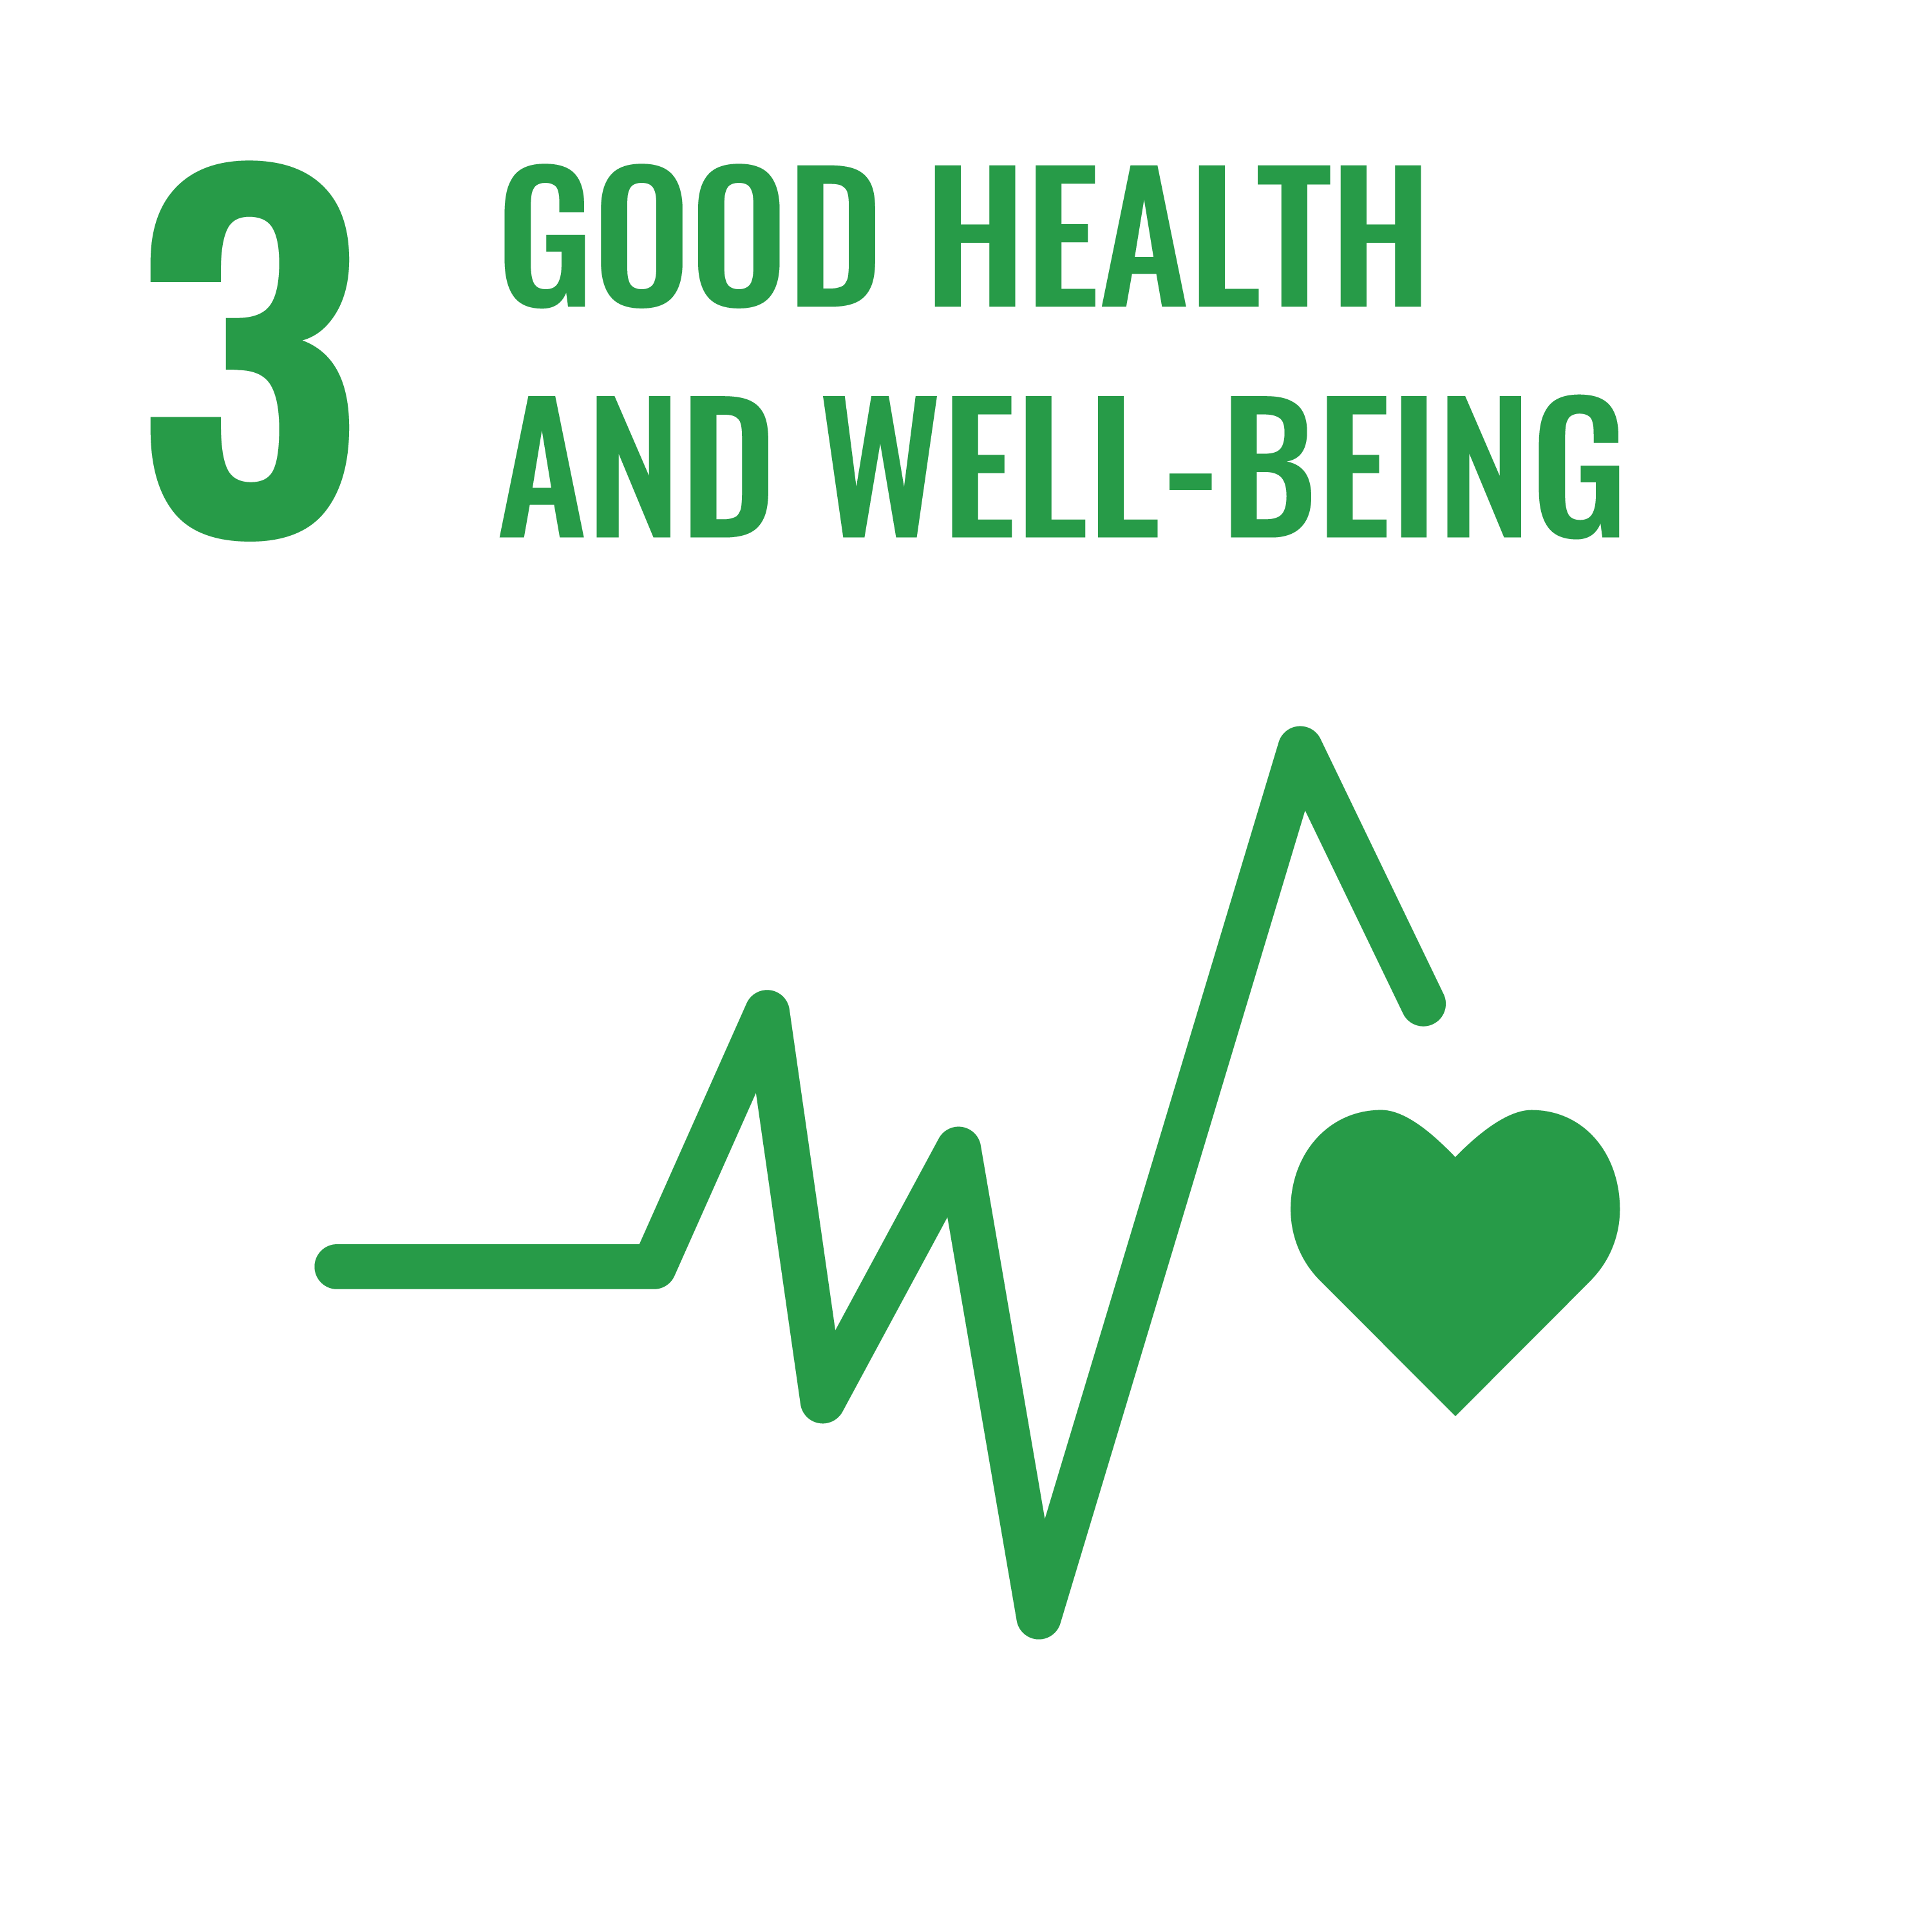
\includegraphics[width=\SDGsize]{Common/SDG_3_GoodHealth.png}~%

\includegraphics[width=\SDGsize]{Common/SDG_9_IndustryInnovation.png}~%
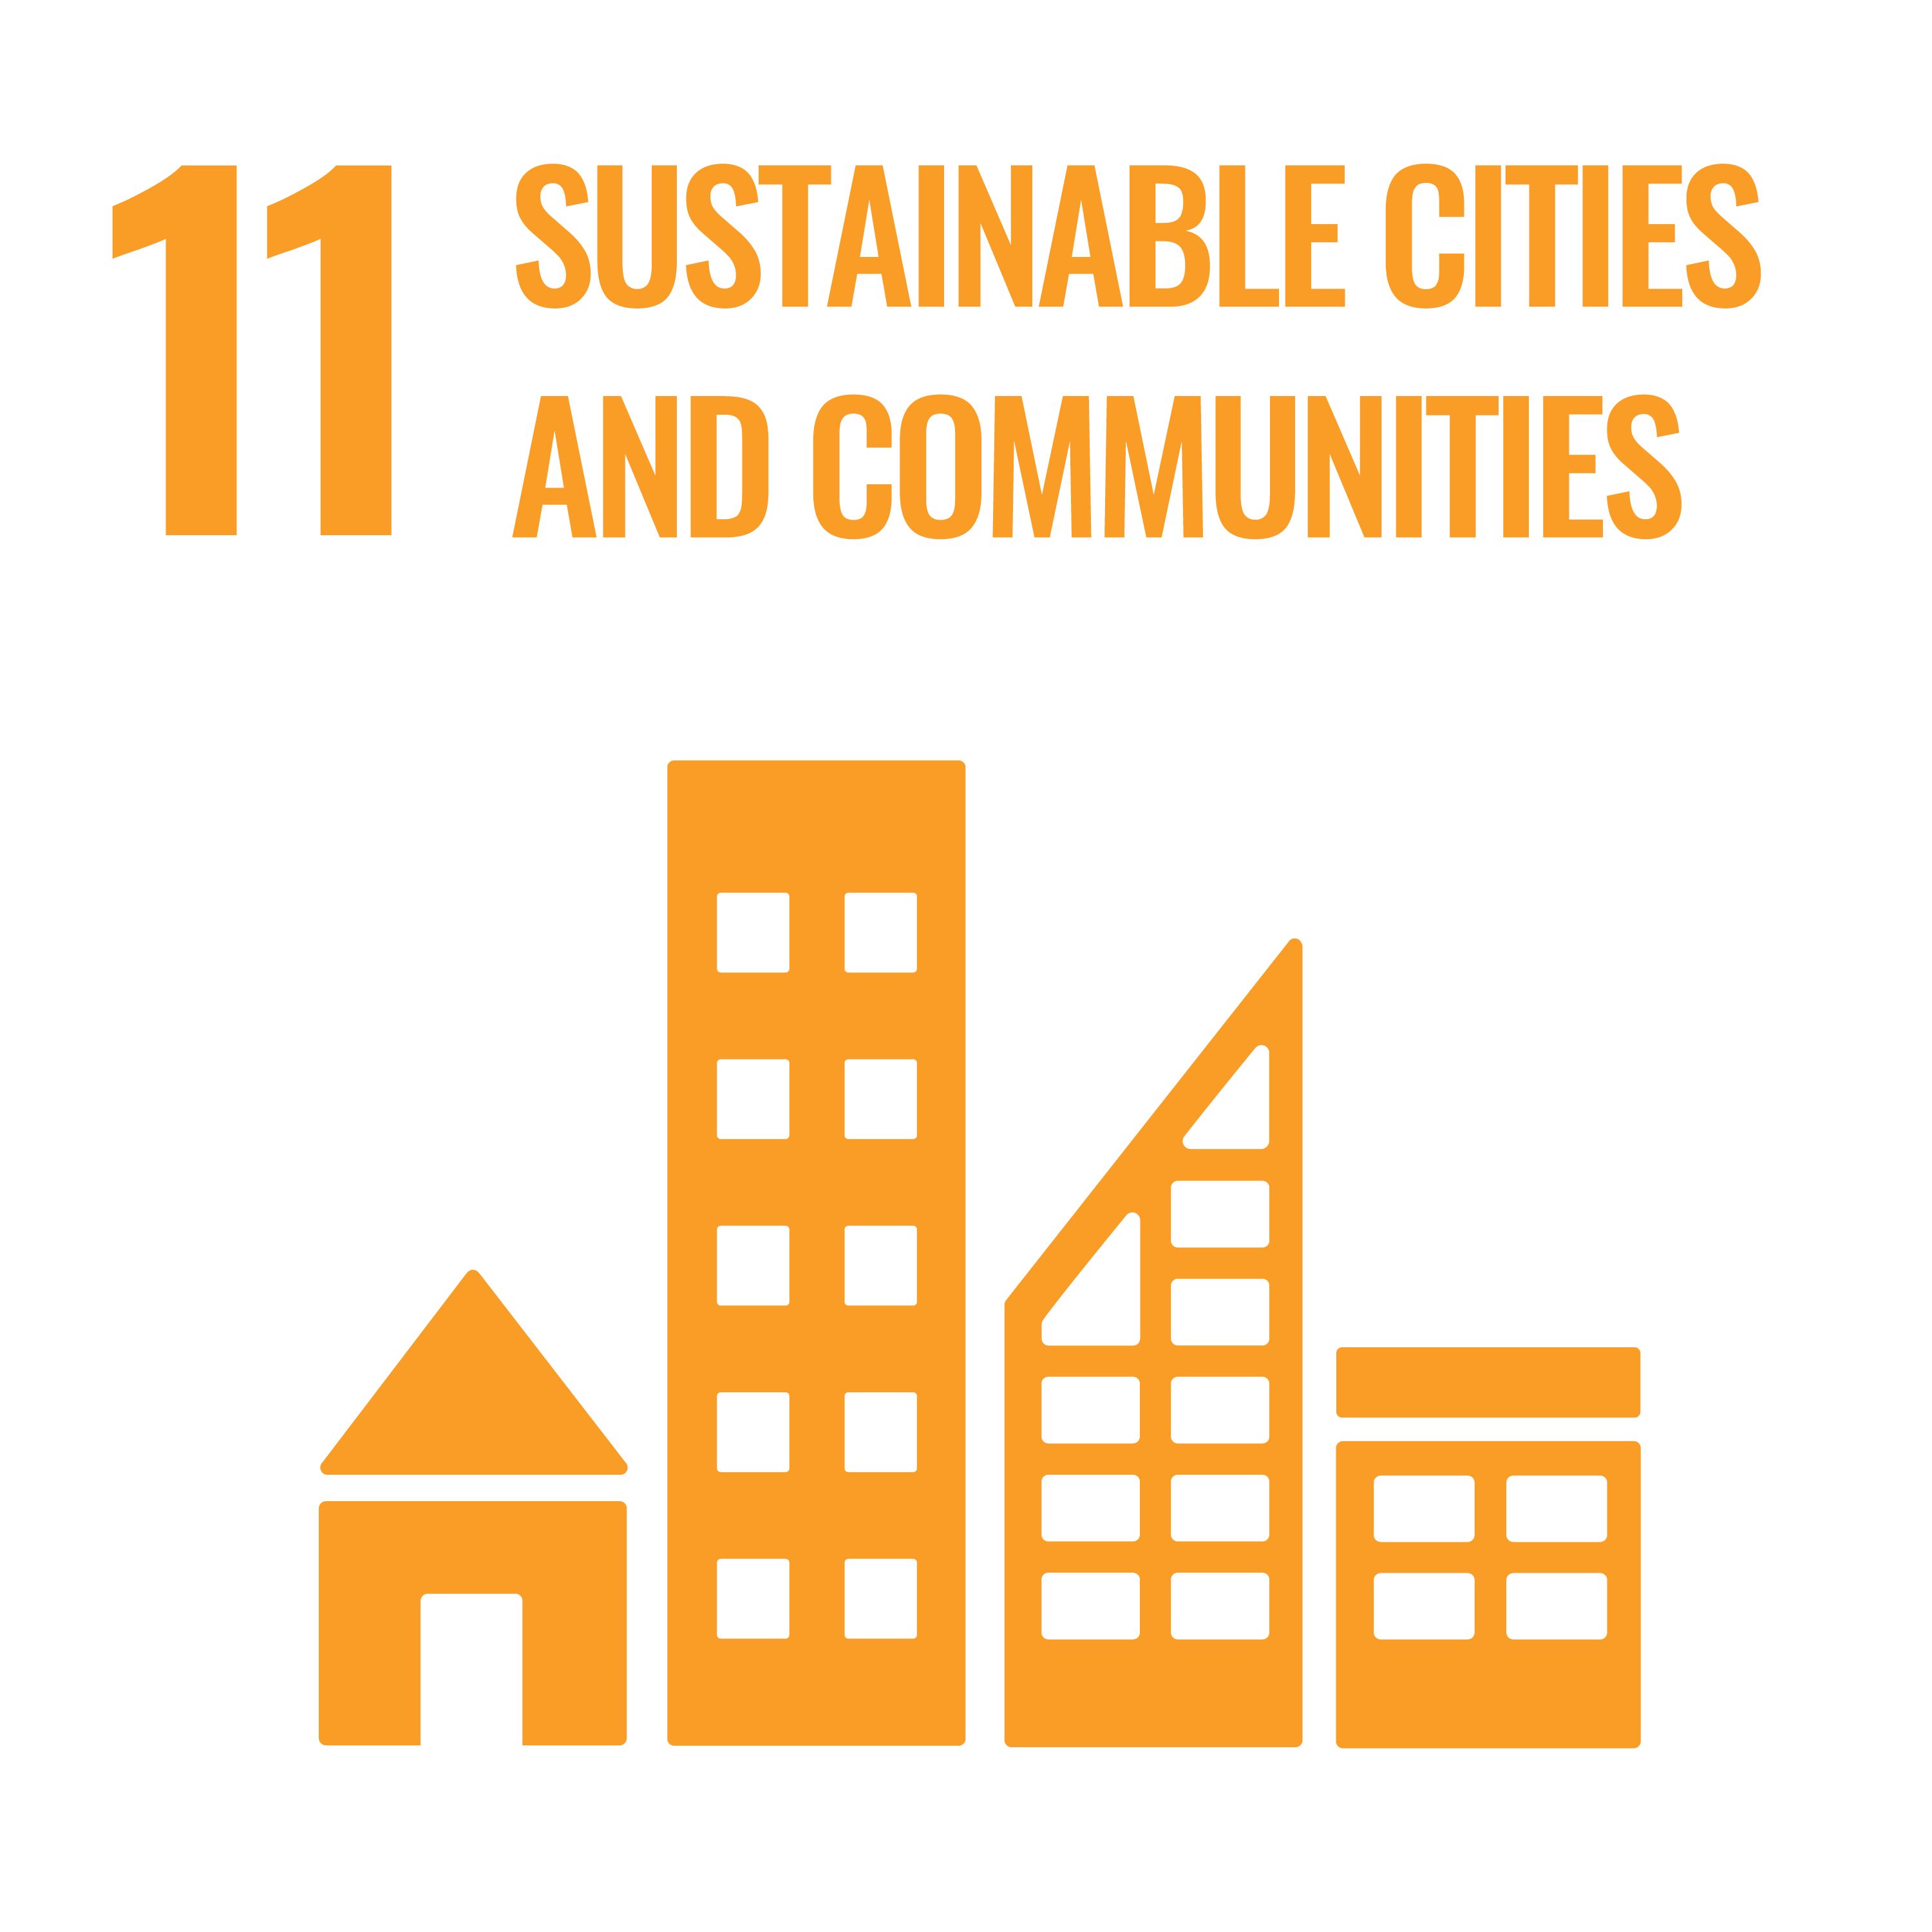
\includegraphics[width=\SDGsize]{Common/SDG_11_SustainableCities.png}~%
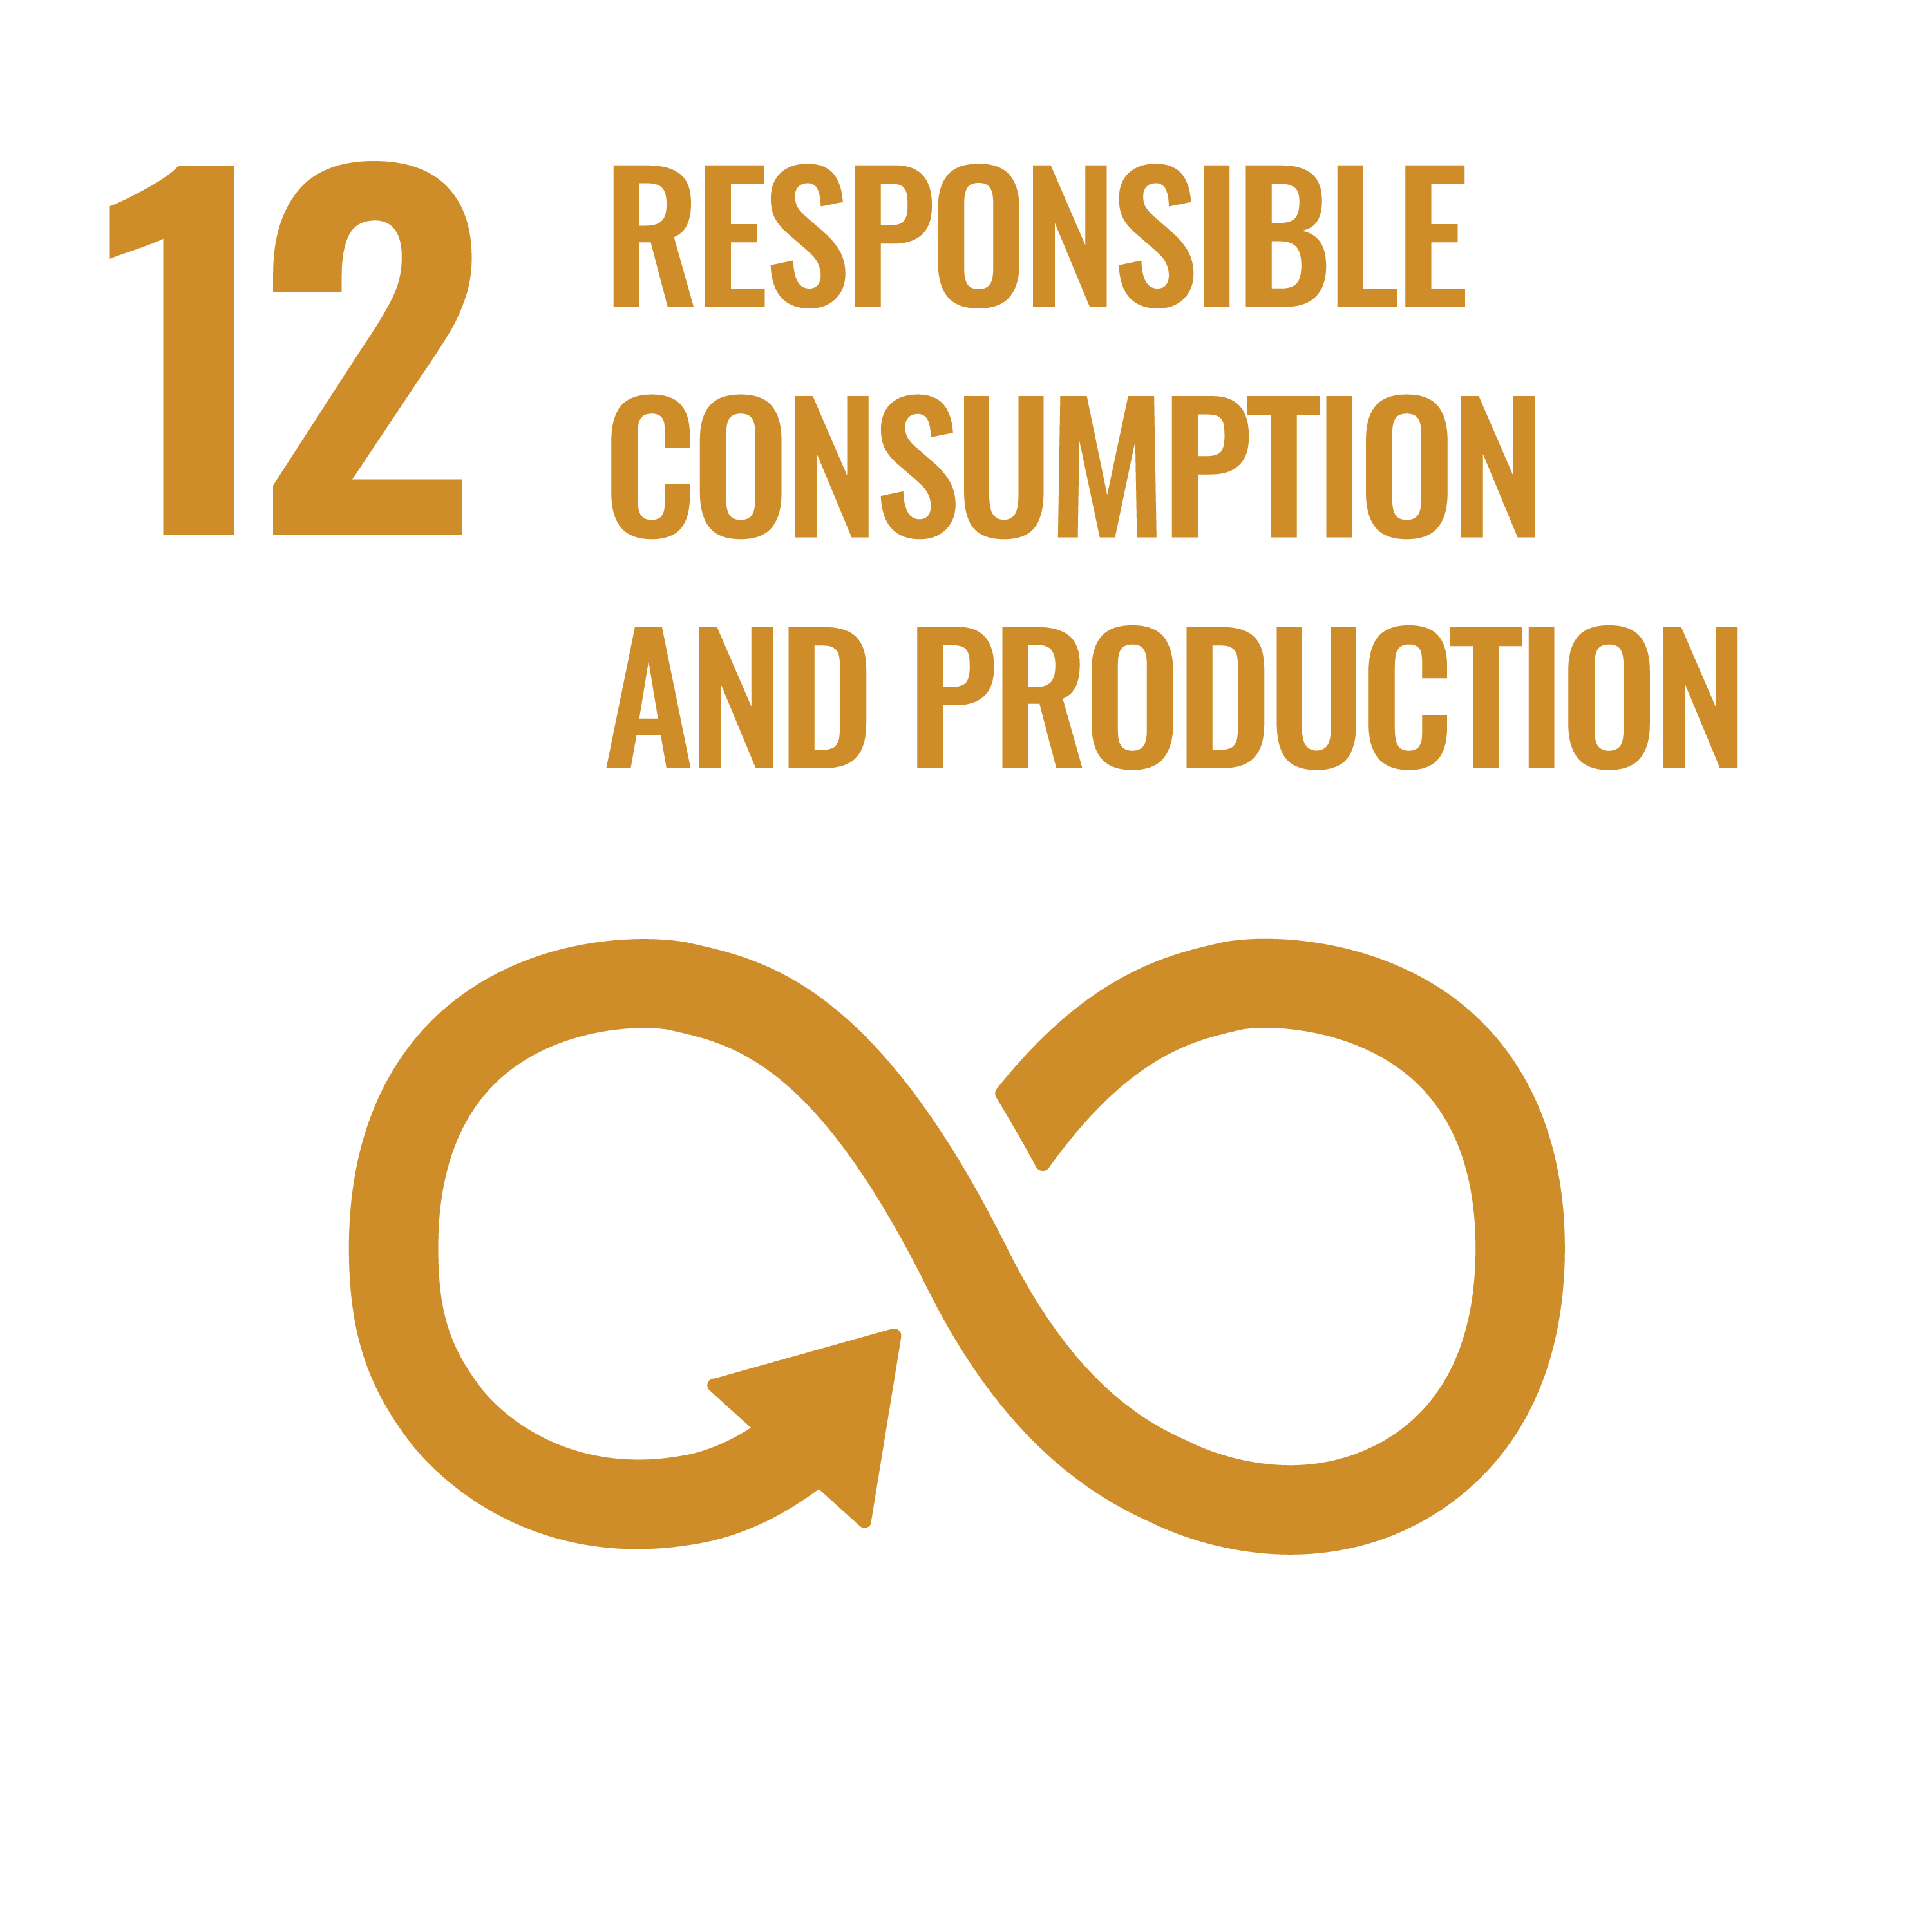
\includegraphics[width=\SDGsize]{Common/SDG_12_ResponsibleConsumption.png}~%
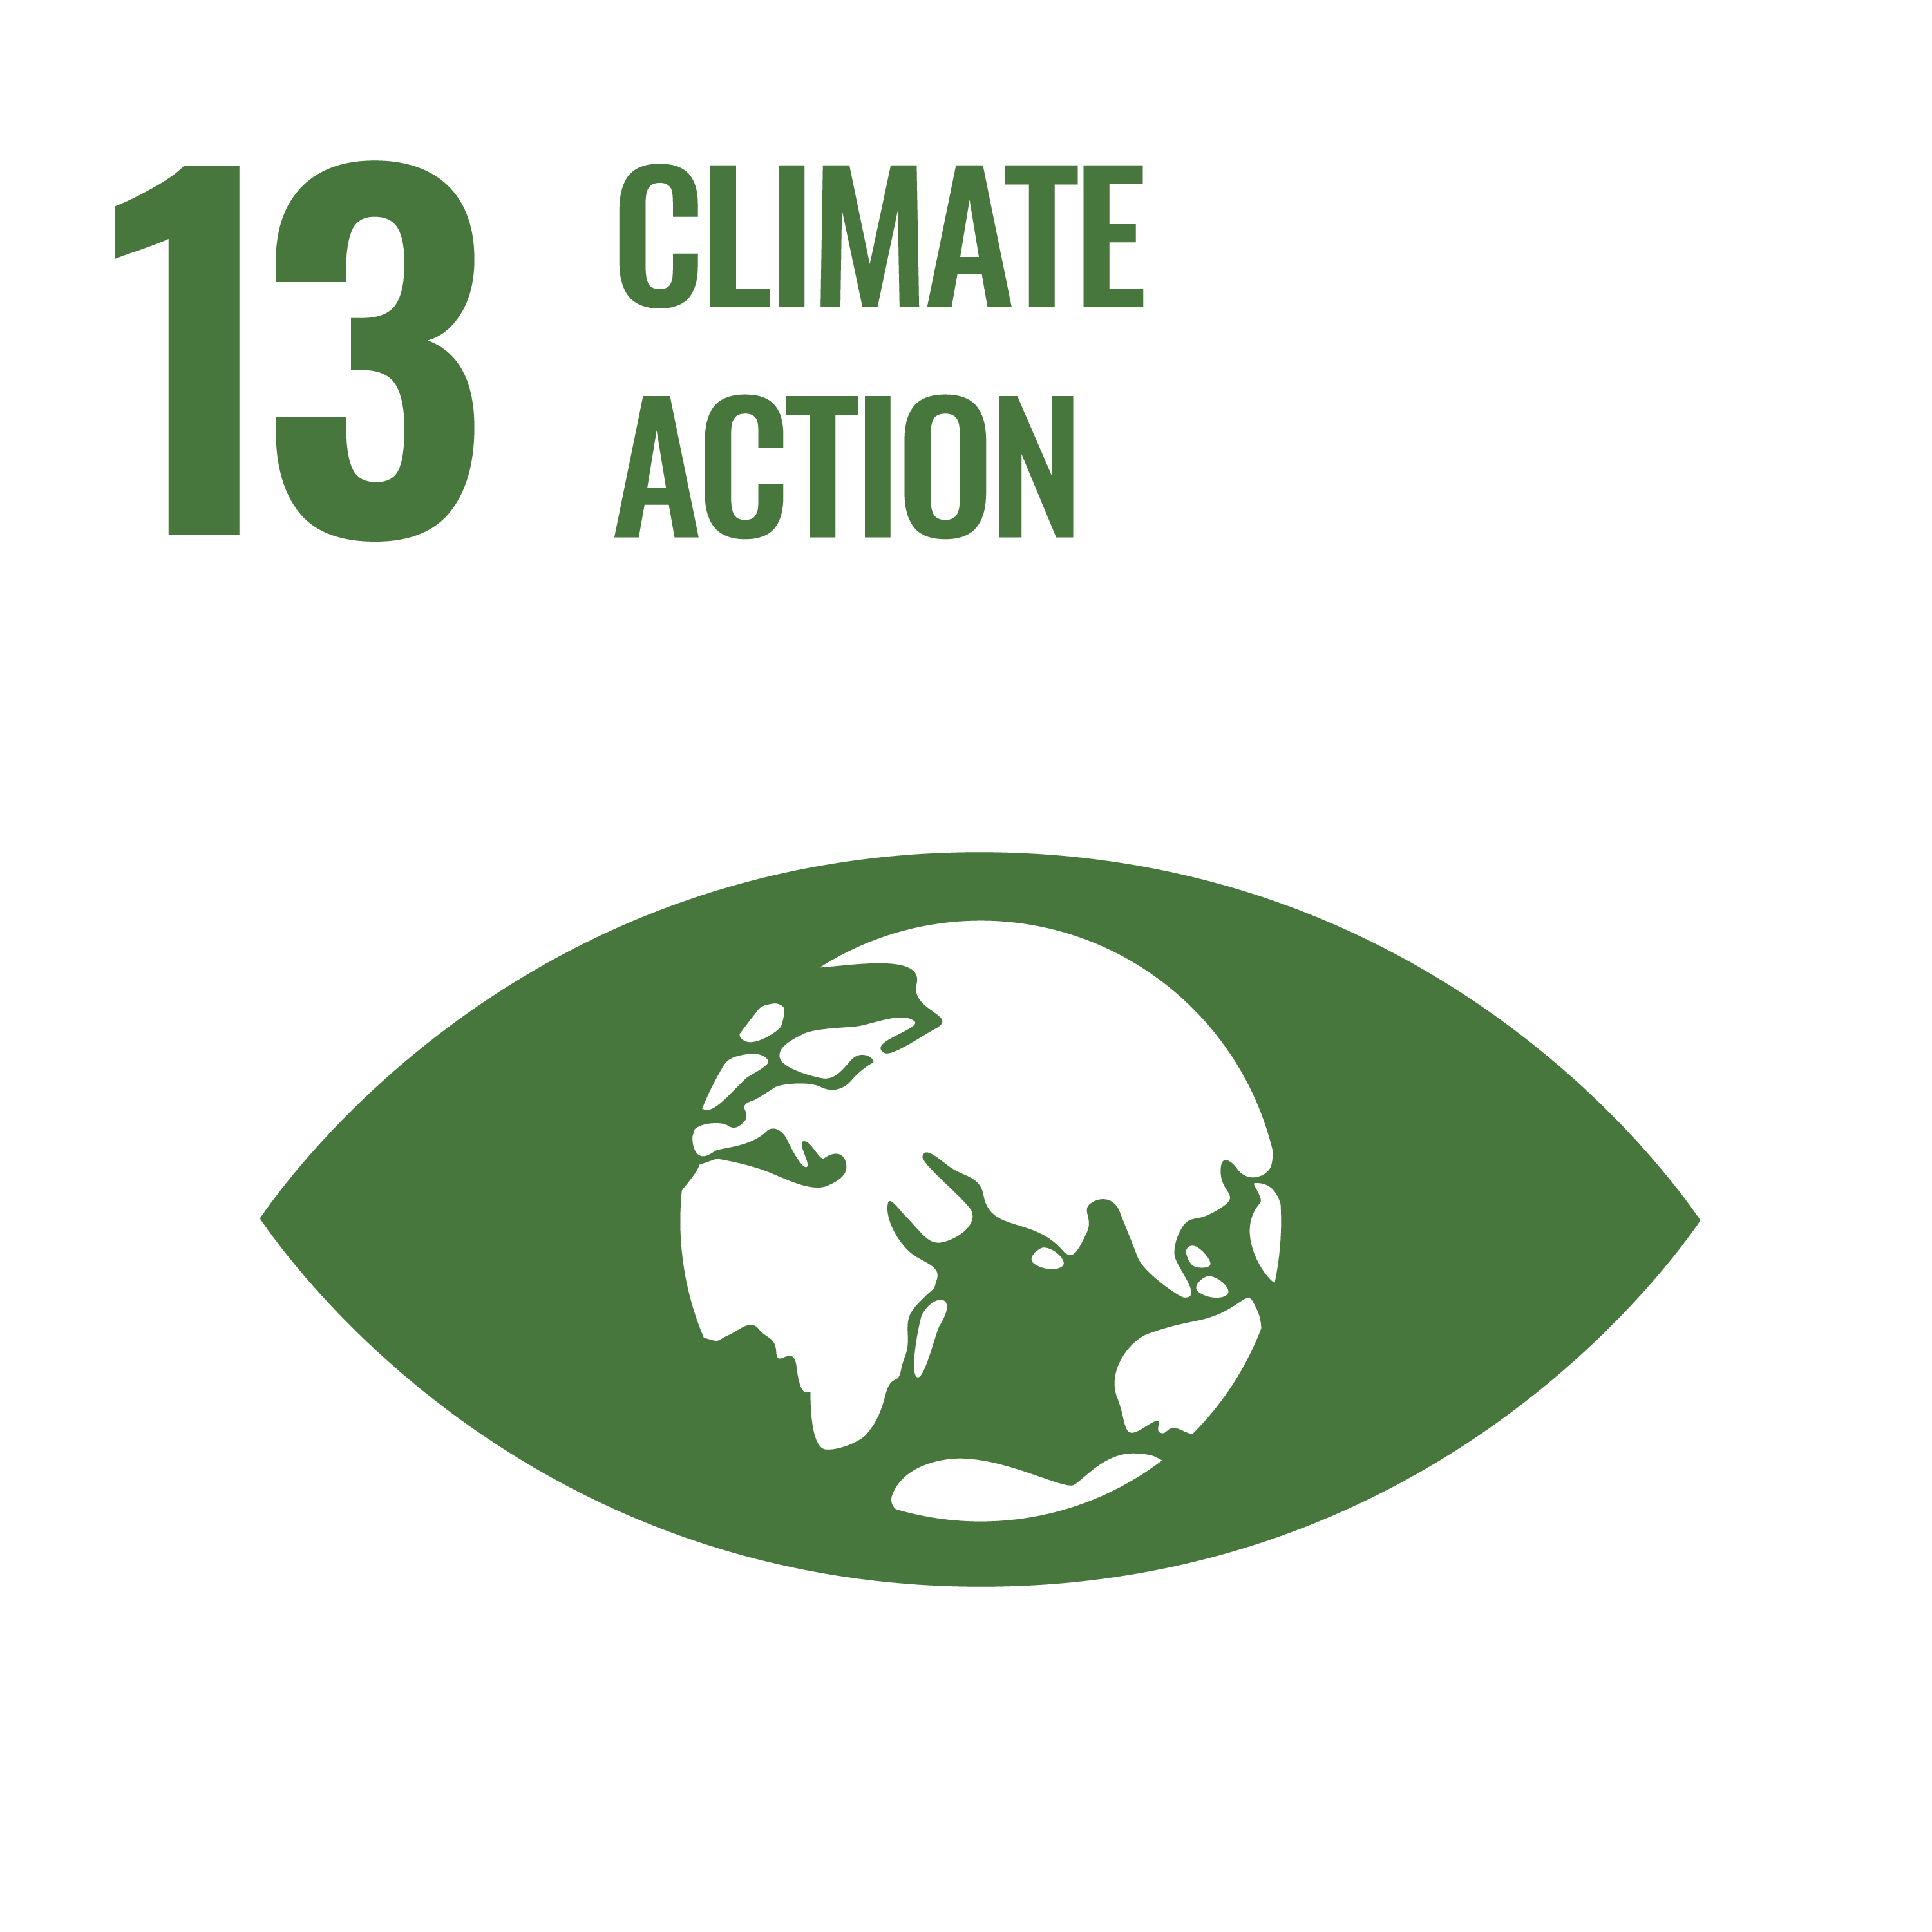
\includegraphics[width=\SDGsize]{Common/SDG_13_ClimateAction.png}
\end{figure}

%%%%%%%%%%%%%%%%%%%%%%%%%%%%%%%%%%%%%%%%

\exSum

\noindent Mobility constitutes a significant portion of the emissions of a \ACR\ researcher.  This includes short daily commutes between the home and the workplace and longer-distance business travel (see \fref{fig:Intro-ComparativeEmissions}).

Transport accounted for almost a fifth of total global emissions in 2016~\cite{OWIDsector}, and is the sector that saw the highest growth in pre-COVID years.  Demand for car, rail, and air transport is expected to continue to increase over time with increasing global population and income levels.

Unsurprisingly, self-powered mobility, such as walking and cycling, are the most carbon-efficient means of transportation, with train travel next best.  A quantitative comparison between these and other options requires further details to be specified, such as the distance travelled, the fuel efficiency of the vehicle used and the number of passengers carried, and the underlying electricity mix for the country of travel.  In the UK for instance, driving alone in a medium-sized petrol-fuelled car yields smaller \acrshort{ghg} emissions than air travel for distances shorter than 1,000 km, whereas flying in economy class beats driving over longer distances~\cite{OWIDtravel} (data taken from Ref.~\cite{BEIS}).\footnote{These estimates include a "radiative forcing" factor of 1.9 for air travel, which account for a larger warming effect due to aeroplanes emitting GHGs high in the atmosphere.} 
For a detailed comparison of emissions due to various forms of transport within France, see \fref{fig:emiMobility}.

When and how we travel, however, are not always free choices, being constrained to some degree by existing transport infrastructure, local geography, our research, finances, and caring responsibilities.  
Universities and \ACR\ institutions, with their large and progressive workforce, can help tip the balance in favour of the more environmentally sustainable option with a judicious combination of policy, incentives, on-site infrastructure and advocacy, as detailed below.

Nevertheless, efforts to limit emissions resulting from travel must be balanced against legitimate needs for mobility: the establishing and maintenance of close collaborative relationships, sharing of research outputs, individual exposure and career development, and travel to research facilities. 
Changes to our travel culture and policies must be implemented so as to benefit and, at the very least, not to worsen barriers to inclusion, by avoiding the disenfranchisement of members of our community such as early career researchers, members of our community from the global south or those otherwise geographically isolated. 

Our current societal infrastructure is set up to facilitate individual travel by car, to the detriment of a large part of the population. Universities, as large employers with a relatively progressive workforce, have the potential to act as instigators of change in this. Making public transport and cycling the preferred options when possible will increase demand for these more sustainable forms of transport and thus encourage cities to improve the infrastructure for them.

\newpage
\begin{reco2}{\currentname}
{
\begin{itemize}[leftmargin=6 mm]
\item Re-assess business travel needs, using remote technologies wherever practicable.
\item Choose environmentally sustainable means of transport for daily commutes as well as unavoidable business travel, amalgamating long-distance trips where possible.
\end{itemize}
}
{
\begin{itemize}[leftmargin=6 mm]
\item Define mobility requirements and travel policies that minimise emissions, while accounting for the differing needs of particular groups, such as early-career researchers or those who are geographically isolated.

\item Re-assess need for in-person meetings, and prioritise formats that minimise travel emissions and diversify participation by making use of hybrid, virtual or local hub participation, and optimising the meeting location(s).

\end{itemize}
}
{
\begin{itemize}[leftmargin=6 mm]
\item Support environmentally sustainable commuting by improving on-site bicycle infrastructure, subsidising public transport and providing shuttle services.

\item Disincentivise car travel where viable alternatives exist, facilitating car pooling and providing on-site charging stations.

\item Incentivise the reduction of business travel, e.g., by implementing carbon budgets with appropriate concessions.

\item Ensure unavoidable travel is made via environmentally sustainable means through flexible travel policies and budgets, and the use of travel agents that offer multi-modal itineraries.  Employ carbon offsetting only as a last resort.

\item Remove any requirement on past mobility as an indication of quality in hiring decisions. 

\item Lobby for improved and environmentally sustainable local and regional transport infrastructure.

\end{itemize}
}
\end{reco2}
\subsection{Commuting}

Changes in commuting patterns are typically affected by life circumstances, including changes in education, employment and residence~\cite{BEIGE2017179}.  The viability of the environmentally sustainable mobility, like walking, cycling and taking the train, depends crucially on characteristics of the home and workplace locations, including the distance between them, and their local environment. These properties are seen to influence the relative importance of commuting and business emissions for different \ACR\ institutions. 

For example, CERN, Fermilab, and ETH Z\"urich have wildly different \CdO\ emission profiles due to personal transportation. While emissions due to commuting were roughly equal to those for business travel at Fermilab, commuting outweighed business travel for CERN, and conversely, business travel swamped commuting emissions for ETH. This reflects the unique environment and characteristics of each these research centres. 

ETH is located in an urban centre and is well connected to the local public transport. In 2008, only 1,700 \tCdOe\ were recorded for commuting, with 7.5 to 10 times larger emissions attributable to business travel (using numbers from 2006--2012). 
It is clear here that the emissions per capita for all staff (including researchers) are significantly smaller than those for Fermilab or CERN. 

The latter two have more rural settings, with a 77\,\% majority of CERN employees commuting by car from France. Fermilab's commuter emissions~\cite{FermilabEnvReport} of about 6,000 \tCdOe\ are approximately on par with business travel emissions,\footnote{In a typical year, Fermilab’s approximately 1,900 staff members commute an average distance of 15.6 miles each way mostly by car. This translates into 5,987 tonnes of \CdO\ when assuming 250 working days per years and using 404~g of \CdO\ per mile as per US~Environmental Protection Agency~\cite{USEPA}. This is only 5\;\% less than Fermilab's emissions from air travel, calculated from 8.2 million (or 42\;\%) fewer miles flown in 2020 using 200~g per air km~\cite{RefAGU}.} whilst CERN quotes 5,836 \tCdOe\ of commuter emissions compared to 3,330 \tCdOe\ business travel emissions for its approximate 4,000 staff members. The small amount of travel emissions compared to emissions from commuting reflects to some extent the status of CERN as scientific centre, where it is expected for other members of the community to travel to and where travel is easier to avoid, also because the experiments are located at CERN. Whilst ETH, Fermilab and CERN face different boundary conditions, all three of them, and \ACR\ institutions in general, should aim to reduce emissions from commuting, even if these contribute to their overall budget to a different degree.

This reduction requires an interplay of institutional and individual actions:\ while institutions cannot force employees to choose more environmentally sustainable commuting habits, they can incentivise them through various measures, from the availability of bicycle-friendly infrastructure such as showers and secured/covered parking to financial incentives for greener transportation. They can also allow employees to avoid long commutes by formalising telecommuting options, which have become more normalised since the start of the COVID-19 pandemic, and use their standing to push local authorities towards better public transit/cycling/carpool infrastructure. Individuals and groups can, on the other hand, push for these actions at the institutional level. Table~\ref{tab:subCommute} collects some means by which ETH, Fermilab and other academic and \ACR\ institutes promote `green' transport. An estimate of the emissions per distance
of different forms of transport in France is presented in \fref{fig:emiMobility}.

%%%%%

\begin{table}
\ra{1.05}
\centering
{\scriptsize
\caption[Measures and subsidies for greener commuting]{Institutional/country-wide measures to encourage sustainable commuting amongst employees. This is a non-exhaustive list; similar initiatives are also offered by other employers.
\label{tab:subCommute}}

\begin{tabular}{m{0.1\textwidth}m{0.22\textwidth}m{0.58\textwidth}}
   \toprule
    Institute &
    Initiative&
    Comments\\ 
    
DESY&
    Reduced-price ticket for public transport for all employees&
    The non-transferable ticket, with a 30\:\% subsidy for employees, is also usable also outside working hours, and allows free network-wide travel for an additional adult and up to 3 children (age 14 and under) on weekends and holidays.
    Requires a subscription of more than 6 months and once
    suspended, a cooling-off period of 9 months is required in order to be eligible for re-subscription (problematic if employee is posted abroad for a few months). With the implementation of the "Deutschlandticket" in Germany, the terms have slightly changed~\cite{DESYsustainableReport2022,hvvJobticket1,hvvJobticket2}.\\
    \midrule
Fermilab&
    Shuttle service
    to and from Chicago Metra trains for all employees &
    Two scheduled connections in the morning and three in the afternoon, on demand at other times, from 06:30 to 18:50. Cost \$2.25 in cash \cite{FNALPace}
    Does not connect to the Metra station serving the fast train to Chicago (Route 59); FNAL do not offer pre-tax public transport ticket purchase.\\
    \midrule
France &
    Public transit subsidy \cite{transitFR} or \EUR{300}/year for all employees who cycle or carpool \cite{mobdouceFR} &
    Honors system for the \EUR{300}/year. 
    The roughly 50\;\% reimbursement on public transport subscription is very helpful, though its adoption depends on
    how well connected each institute is.\\
    \midrule
Germany & 
    General tax reimbursement for commuting depending on distance & 
    For each km travelled to work \EUR{0.30} is deducted from the taxable income (\EUR{0.38} per km above 21 km per one way starting from 2022) \cite{GermanyTax}. 
    This is independent of the means of transport and also applies to cyclists or pedestrians, but is more advantageous for people with longer commutes who are less likely to use eco-friendly means of transport. \\
    \midrule
University of Sheffield  &
    Bike to work scheme for all employees & Possibility to borrow an e-bike (or a bike) for free for 2 months in order to test commuting by bike.
    Ability to rent bikes throughout the semester and to buy reconditioned bikes. Over 1,400 cycle parking spaces available throughout campus and at the residences.
    Service to provide free bike checks and at-cost servicing and repairs for staff and students funded by the university.
    (All UK universities.) Financial help to buy an e-bike. (However, this is based on reducing the university's financial contribution to the pension scheme over a set amount of time.)~\cite{shefbike}
    \\
   \bottomrule
   
\end{tabular}}
\end{table}

%%%%%

\clearpage

\begin{figure}
    \centering
    \caption[Mobility emissions]{GHG emissions
for different means of transport (in g\CdOe\ per km).  Emissions from electricity and vehicle production as well as fuel combustion are included.  All data is for 2019--2020, and comes from the database of Ref.~\cite{labos1p5} --- see, in particular, Ref.~\cite{labos1p5emi} --- and assumes the electricity comes from the French grid, which is a factor of 10 less carbon-intensive than other countries~\cite{OWDintensity}.  For a comparison with the UK, see Ref.~\cite{OWIDtravel}. Note that emissions from personal transport do not scale linearly with number of passengers.
\label{fig:emiMobility}}
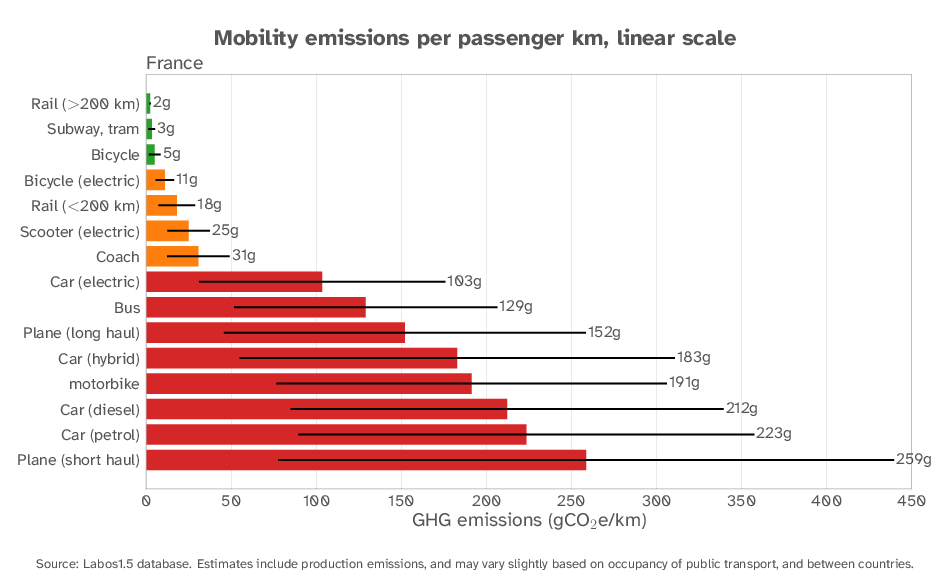
\includegraphics[width=\textwidth]{Sections/Figs/Travel/MobilityEmissionsLinear.png}
\end{figure}
%%%%%


\subsection{Business Travel}

A global scientific endeavour such as \ACR\ will mandate some amount of long-distance travel, e.g., to experimental sites, or to build close working relationships.  However, the current academic culture which rewards hyper-mobility is neither environmentally sustainable, nor equitable to all scientists.  Visa rules and prohibitive long-haul travel costs can make participation in conferences extremely challenging, especially for researchers from the Global South. Moreover, the freedom to travel can be heavily restricted for people with disabilities, health impairments or caring responsibilities. For example, the burden of childcare is still unequally distributed, and this burden falls predominately on female shoulders~\cite{McCarthy}.

Emissions from commercial aviation is a long-recognised problem, contributing 2.5\% of \CdO\ emissions and 3.5\% of ‘effective radiative forcing’ (a closer measure of aviation's impact on warming as explained above)~\cite{Rit20} in 2018.  Note that the majority of these emissions derive from the one-tenth of the world’s population that can afford air travel.  Almost all \ACR\ scientists belong to the 4\% of the population taking international flights, and many fall within the 1\% classified as the most frequent flyers~\cite{GOSSLING2020102194}.  These statistics highlight the inequalities inherent in travel emissions generally.

More troubling is that global aviation statistics belie the significance of business travel emissions for many \ACR\ researchers, which are comparable to, and in some cases even dwarf, their direct and indirect emissions (see \fref{fig:Intro-ComparativeEmissions}).  This is clearly in tension with the push to net zero emissions, particularly given that we do not expect the aviation sector to decarbonise at the same rate as the rest of the transport sector.

Emissions related to conference travel have been studied in detail and dominate conference-related emissions~\cite{Spinellis, nature_better_confs}, contributing annual emissions equivalent to the total annual transportation emissions for Geneva (800 kilotonnes \CdO).  However, the \CdO\ emissions for a single conference trip amount to about 7\% of an average individual’s total \CdO\ emissions. This might be even worse for \ACR\ researchers, for whom frequent trips to experimental sites and meeting venues to undertake international collaborations are common.  See also emissions estimates for business travel of members of the LHCb collaboration in \csref{case:LHCb}.

Discussions about curbing business travel are highly charged, as active engagement with other members of the scientific community is integral to scientific practice. Any changes that we make to \ACR\ travel culture have to be considered in the context of other aspects of our working practices, such as hiring decisions, where any curbs on travel may, \eg disproportionately impact early career researchers. At the same time, the reprioritisation of business travel and a move toward a greater share of virtual/hybrid formats can have a positive impact both on the climate and on inclusivity.

For necessary travel, sustainable alternatives to air travel should be prioritised where possible, keeping in mind that the increased travel time and costs of sustainable travel as compared with air travel could make this choice difficult for researchers with caregiving responsibilities, or limited travel budgets.  In \csref{case:traveltoCERN}, we compare emissions, travel time and cost of different modes of travel to CERN, from various starting points within Europe, for CMS week in January 2022.  \ACR\ institutions and funding bodies are beginning to implement more sustainable travel policies, including travel top-ups for green travel; we highlight two examples in \bpref{bp:Erasmus} and \bpref{bp:DESY_travel}.

If the community is to rethink this travel culture and move toward more hybrid/virtual modes of engagement, we must recognise that these require additional planning to maximise engagement, which amounts to much more than streaming the in-person event format (see~\csref{cs:CfH}). It is also important to appreciate that virtual participation requires an internet-ready device and stable connection, and devices with which to connect, which may not be universally available in lower income countries. A possible remedy for this might be the concept of hub conferences, where the conference has several locations spread globally (\eg Ref.~\cite{Parncutt}).  In \csref{case:ICHEP}, we study travel emissions and participation in the context of the last 5 ICHEP conferences, and assess the reduction in emissions from optimising the conference location, moving to a hub model, or hybrid/virtual forms of attendance.

%%%%%

\begin{casestudy}[Sustainable travel to CERN\label{case:traveltoCERN}]{Sustainable travel to CERN}%
The itineraries in \tref{tab:CERNtravel} were found for travel to CERN for, e.g., CMS week, 24$^\text{th}$--28$^\text{th}$ January 2022, as found on 30$^\text{th}$ November 2021\footnote{Prices and carbon footprint rounded to nearest whole number.  For prices not given in euros, currency conversions were made using Google currency converter.  Carbon footprints for one-way travel were calculated using Ref.~\cite{ecopassenger} and then doubled, using all default assumptions, except for toggling on the climate factor for flights.  Precise departure and arrival information was not used for calculation of the flight footprint.  Since some airports are not included as possible destinations, the footprint was calculated from the central train station in the origin city to the central train station in the destination city, and the footprint of travel to the airport is assumed negligible (in comparison to the flight).  Train fares quoted are for the most convenient train journeys from the central station in the origin city to the central station at the destination.  For longer journeys, preference was given to itineraries with overnight trains to maximise efficiency per euro spent, assuming savings on an additional night in a hotel.  For all overnight trains, quoted prices include reservation in shared sleeper cabin. Female-only occupancy can be specified. Note that in many cases there may be a limited number of 'super saver' tickets that are available for purchase ahead of time.  Air fares were for the ‘best’ option available on Skyscanner~\cite{skyscanner}, with inbound flight arriving in time for an assumed midday start of meetings at CERN, and outbound flight departing after 15:00 hours on Friday.  Flight prices were taken directly from the airline where possible, and include a standard-sized cabin bag, but not necessarily a checked bag.  Durations include flight time only and do not include airport check-in times.}.  Although emissions were significantly smaller for rail travel as compared with travel by car or air, as expected, this must be weighed against the increased travel time, and in many cases, cost of rail travel.  Note that the air travel times are underestimated as they do not include travel to the airports which are usually distant from the city centres, or the usual buffer time required for check-in and security formalities.  For itineraries that include sleeper trains, the additional cost of the train could offset a night's hotel accommodation at origin or destination.
\end{casestudy}

%%%%%

\begin{landscape}
{\tiny
\centering
\ra{1.05}
\extrarowheight=\aboverulesep
\addtolength{\extrarowheight}{\belowrulesep}
\aboverulesep=0pt
\belowrulesep=0pt
\captionsetup{type=table}
\caption[Comparison of modes of travel to CERN from different origins]{Comparison of modes of travel to CERN from different origins.}
\label{tab:CERNtravel}
\begin{tabular}{@{\kern\tabcolsep}p{1.8cm}>{\baselineskip=10pt}p{1.5cm}>{\RaggedRight\arraybackslash\baselineskip=15pt}p{3cm}>{\baselineskip=15pt}p{2.0cm}>{\baselineskip=15pt\RaggedRight\arraybackslash}p{11cm}>{\baselineskip=10pt}p{1.1cm}>{\baselineskip=10pt}p{1.5cm}c@{}}
\toprule
\cellcolor{gray!20}Distance &
\cellcolor{gray!20}Origin &
\cellcolor{gray!20}Mode of Transport &
\cellcolor{gray!20}Travel time (one way) &
\cellcolor{gray!20}Itinerary&
\cellcolor{gray!20}Price (EUR)&
\cellcolor{gray!20}Emissions (kg \CdOe)
\\ \cmidrule{1-7}
  
$<$600 km&
Paris  & 
Train  &
3h15     &
\textbf{Out:} Mon 24th 08:18 - 11:29 
\textbf{In:} Fri 28th 14:29 - 17:42     & 
178    & 
\noindent\color{green}{25}  
\\ \cmidrule{3-7}
&  & 
Flight 
ORY-GVA& 
$\sim$1 hr& 
\textbf{Out: }Mon 24th 08:20 - 09:25 
\textbf{In:} Fri 28th 19:05 - 20:15& 
98& 
235
\\  \cmidrule{3-7}
&  & 
Car&
5h42&
& &
116 \\  \cmidrule{1-7}
$>600$ km& 
\cellcolor{gray!10}Hamburg&
\cellcolor{gray!10}Train (2 changes)&

\cellcolor{gray!10}$\sim$13.5 hrs&
\cellcolor{gray!10}\textbf{Out:} Sun 23rd 20:50 - 10:18 (+1 day)
\textbf{In:} Fri 28th 18:15 - 07:54 (+1 day) &
\cellcolor{gray!10}258&
\cellcolor{gray!10} {\noindent\color{green} 46} \\ \cmidrule{3-7}
&\cellcolor{gray!10} &
\cellcolor{gray!10}Flight
HAM-GVA\linebreak
(1 change)&
\cellcolor{gray!10}$\sim$3 hrs&
\cellcolor{gray!10}\textbf{Out:} Mon 24th 07:00 - 10:10
\textbf{In:} Fri 28th 19:10 - 22:35&
\cellcolor{gray!10}261&
\cellcolor{gray!10}497\\ \cmidrule{3-7}
&\cellcolor{gray!10} &
\cellcolor{gray!10}Car&
\cellcolor{gray!10}9h50&
\cellcolor{gray!10}&\cellcolor{gray!10}
 &\cellcolor{gray!10}
225 \\ \cmidrule{2-7}
&
London&
Train
(2 changes out; 1 change in)&
$\sim$8  hrs&
\textbf{Out:} Sun 23rd 15:31 - 23:29
\textbf{In:} Fri 28th 15:30 - 22:30&
288&
{\color{green} 25}\\ \cmidrule{3-7}
& &
Flight  
LTN-GVA&
1h40&
\textbf{Out:} Mon 24th 08:00 - 10:45
\textbf{In:} Fri 28th 21:40 - 22:20&
80&
402\\ \cmidrule{3-7}
& &
Car&
8h32&
& &
 196 \\ \cmidrule{2-7}
  &
\cellcolor{gray!10} Rome&
\cellcolor{gray!10}Train 
(1 change) &
\cellcolor{gray!10}$\sim$8.5 hrs &
\cellcolor{gray!10}\textbf{Out:} Sun 23rd 15:25 - 23:54 
\textbf{In:} Friday 28th  13:39 - 21:40&
\cellcolor{gray!10}238&
\cellcolor{gray!10} \noindent{\color{green} 70}\\\cmidrule{3-7}
& \cellcolor{gray!10}&
\cellcolor{gray!10}Flight
 FCO-GVA &
\cellcolor{gray!10}1h30&
\cellcolor{gray!10}\textbf{Out:} Mon 24th 09:00 - 10:30
\textbf{In:}  Friday 28th 18:45 - 20:20&
\cellcolor{gray!10}77&
\cellcolor{gray!10}392\\ \cmidrule{3-7} 
&\cellcolor{gray!10} &
\cellcolor{gray!10}Car&
\cellcolor{gray!10}$\sim$8 hrs&
\cellcolor{gray!10}&\cellcolor{gray!10} & 
\cellcolor{gray!10}183 \\ \cmidrule{2-7}
&
Barcelona&
Train&
7-8 hrs&
\textbf{Out:} Sun 23rd 08:15 - 16:35
\textbf{In:} Fri 28th 12:35 - 19:32&
147&
{\color{green} 18}\\  \cmidrule{3-7}
& &
Flight
BCN - GVA&
$\sim$1.5 hrs&
\textbf{Out:} Mon 24th 08:40 - 10:20
\textbf{In:} Fri 28th 17:00 - 18:25&
83&
370\\  \cmidrule{3-7}
& &
Car&
7 hrs&
& &
164 \\  \cmidrule{1-7}
$>1200$ km &
\cellcolor{gray!10}Warsaw&
\cellcolor{gray!10}Train
(2 changes)&
\cellcolor{gray!10}22.5 - 24.5 hrs&
\cellcolor{gray!10}\textbf{Out:} Sat 22nd  19:49 - 18:18 (+1 day) 
\textbf{In:} Fri 28th  18:42 - 19:15 (+1 day)&
\cellcolor{gray!10}319& 
\cellcolor{gray!10} \noindent{\color{green} 176}\\  \cmidrule{3-7}
&\cellcolor{gray!10} &
\cellcolor{gray!10}Flight 
WAW-GVA&
\cellcolor{gray!10}2h20&
\cellcolor{gray!10}Out: Mon 24th  07:20 - 09:40 
In: Fri 28th  19:45 - 21:55&
\cellcolor{gray!10}185&
\cellcolor{gray!10}531\\  \cmidrule{3-7}
&\cellcolor{gray!10} &
\cellcolor{gray!10}Car&
\cellcolor{gray!10}12.5 hrs&
\cellcolor{gray!10}&\cellcolor{gray!10} &
\cellcolor{gray!10}398\\\bottomrule
\end{tabular}
}
\end{landscape}

\clearpage

%%%%%%%%%%%%%%%%%%%%%%%%%%%%%%%%%%%%%%%%%%%%%%%%%%

\begin{casestudy}[Comparative study of travel emissions for ICHEP conferences (2012--2020)\label{case:ICHEP}]{Comparative travel emissions for ICHEP conferences}% 
Based on the study of the annual meetings of the American Geophysical Union (AGU) in Ref.~\cite{RefAGU} and the methodology and software tools employed therein, we undertake a survey of the past five editions of the International Conference for High Energy Physics (ICHEP) with the aim of assessing the GHG emissions of conference travel to ICHEP, as well as the (geographical) diversity of participants.

ICHEP is a biannual conference with a large and steadily growing participation, of order 1,000 researchers, and a location that alternates mainly between Europe, America and Asia.  We study the 5 most recent instances, with locations in Melbourne, Australia (2012), Valencia, Spain (2014), Chicago, United States, (2016), Seoul, Korea (2018) and Prague, Czech Republic (2020, fully virtual).  At the time of writing the 2022 conference, to be held in Bologna, had not yet begun.

\paragraph{Methodology}

Participant details were taken from the Indico conference system registration pages~\cite{indico}. The departure location for each participant was assumed to be the city of their affiliation, save for cases where it was clear that the participant was based in Geneva, as is often the case for members of LHC collaborations. Direct travel to and from the conference was assumed.  Distances were calculated as the great circle distance using coordinates obtained with Nominatim from the OpenStreet Map data base. Rail, car or bus travel was assumed for all journeys with distances of less than 400 km, with air travel assumed for longer distances.  `Short-haul' was defined as travel distances of less than 1,500 km; distances up to 8,000 km are `long-haul' and longer distance still were classified as `super long-haul'.

\begin{figure}
{\scriptsize
\ra{1.1}
\captionsetup{type=table}
\caption[Total number of participants of recent ICHEP conferences and the GHG emissions per participant]{Total number of participants of recent ICHEP conferences and the GHG emissions per participant.
The corresponding numbers for the AGU Fall Meeting~\cite{RefAGU} are shown for reference.}
\label{tab:icheppart}
\begin{tabular}{@{}p{2.3cm}>{\baselineskip=10pt}p{1.8cm}>{\baselineskip=10pt}p{1.5cm}>{\baselineskip=10pt}p{1.5cm}>{\baselineskip=10pt}p{1.5cm}>{\baselineskip=10pt}p{1.4cm}>{\baselineskip=10pt}p{1.7cm}c@{}}\toprule
&AGU Fall Meeting 2019 & 
ICHEP Melbourne 2012 & 
ICHEP Valencia 2014 &
ICHEP Chicago 2016 & 
ICHEP Seoul 2018 &         
ICHEP Prague 2020 (virtual) \\ \cmidrule{2-7}
    
Number of participants&
24009       & 
764     &
966     &
1120    & 
1178    & 
2877    \\ \midrule

GHG emissions per participant [kg \CdOe]     & 
2883     & 
8432     & 
1902     & 
2699     & 
2648     & 
0 \\
\bottomrule
\end{tabular}}
\end{figure}

Table~\ref{tab:icheppart} shows the average GHG emissions per participant for the ICHEP editions alongside those for the 2019 AGU Fall Meeting for reference. With the exception of the 2012 Melbourne edition of ICHEP, the per capita emissions were significantly lower for ICHEP, which is a ``travelling'' conference, as compared with the stationary AGU Meeting, which always takes place in San Francisco. This indicates that moving a conference series between continents naturally reduces the travel-related emissions as participants tend to wait for the conference to be held near them to make the trip.  Comparing the geographical distribution of home institutes for each conference reinforces this conclusion.  Note that ICHEP Melbourne (2012) was the first and only ICHEP conference taking place in Oceania.

The emissions for two typical ICHEP conferences, one in Europe (Valencia) and the other further removed, in Asia (Seoul) are displayed as a function of travel distance in \fref{fig:EmmPerDistance} below.  Due to the remote nature of the conference location, a large fraction of attendees at the Seoul conference had to fly super-long-haul to get there, giving rise to the majority of the emissions.  Emissions for the remaining half of the attendees was nearly negligible.  This was not the case for Valencia, where as many attendees travelled short haul travel or less.  It is also clear that the bulk of the emissions is due to long-haul or super-long-haul air travel.

\begin{figure}
    \captionsetup{type=figure}
    \subfloat{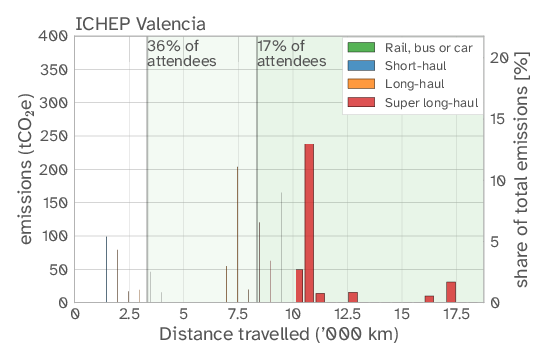
\includegraphics[width=.49\textwidth]{Sections/Figs/Travel/EmissionsDistanceVLC.png}}
    \subfloat{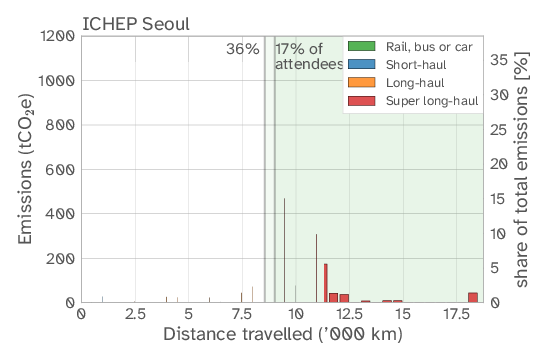
\includegraphics[width=.49\textwidth]{Sections/Figs/Travel/EmissionsDistanceICN.png}}\\
    \caption[Emissions per distance for two different ICHEP editions]{Emissions per distance for ICHEP Valencia and ICHEP Seoul shown in \tCdOe\ (left axis) and as share of the total emissions. Additionally, the emissions caused by the 17~\% and 36~\% of participants travelling furthest are shaded in green.}\label{fig:EmmPerDistance}
\end{figure}

Reference~\cite{RefAGU} investigated possible optimizations of the conference location for the given participant distribution in order to reduce emissions.\footnote{Optimizations were carried out with a grid spacing, and hence resolution, of 1 degree longitude and latitude}  Note that this is a slightly artificial construction because of the basin of attraction phenomenon discussed above, where participant distribution is self-selecting, based on the conference location. Unlike the AGU example, where moving the conference location to the middle of the country, rather than on a coast, significantly decreased the travel-related emissions, we found that the ICHEP locations were already pre-optimised, and further optimisation yielded at most a 10.2 \% reduction of GHG emissions.  (The real outlier again was Melbourne, where the majority of participants had to fly super long-haul, and for which a 70.7 \% reduction would be achievable given the same participants by changing the location).  If instead we optimised the location using participants from all 5 ICHEPs, the optimal location would be close to Amsterdam.

Further emissions reductions are only possible with a hub-based conference, and mandatory virtual participation above a certain distance from the hubs. Ref.~\cite{RefAGU} trialled hubs in Chicago, Seoul and Paris, with virtual attendance for all participants with origins greater than 2000 km from the hubs.  Having found that Chicago, Seoul and Paris were not far from the optimal locations for the respective ICHEP conferences, we did the same, for the total ICHEP participation over the 5 conferences.  Simply using a 3-hub model can reduce the carbon footprint of the conference to around 15--35 \% of a traditional one.  Adding compulsory virtual participation for more distant participants reduces the carbon footprint further by 5--15 \% of a traditional conference with 10--25 \% of the participants attending virtually.  As a test case, and without any prior optimization, we chose Rio de Janeiro, Johannesburg, and Kolkata as alternative hubs. This, however, increased virtual participation to 95 \%¸ mainly due to the strong European participation in HEP and the remoteness of Johannesburg from Western Europe. Switching Paris for Johannesburg reduced the footprint to about 10 \% of the nominal one, with 40\% of participants attending virtually. While the virtual fraction is still relatively high, it might be acceptable in a bid to include more remote HEP communities (like Melbourne) while keeping the emissions low.

Finally, one might expect a fully virtual conference to be more inclusive than in-person ones, especially for underserved participants, such as those with care-giving responsibilities, limited travel funding, or visa problems.  We studied this by classifying participants by the human development index (HDI)~\cite{hdiref} of their country of affiliation, and dividing them into four categories (low, medium, high and very high HDI).\footnote{Examples of countries with very high HDI are Norway,  Malaysia, Kuwait and Serbia, high HDI are \eg Trinidad and Tobago, Albania, Egypt and Vietnam. Medium HDI countries include Morocco and Pakistan, while low HDI countries are \eg Nigeria, Chad and Niger. A brief overview of the categories can be found in Ref.~\cite{hdiref}.}  The share of participants in these categories for each of the ICHEP conferences is shown in \fref{fig:DevelopmentIndex}. Indeed, in addition to enjoying the largest number of participants (by a factor of 2), the virtual ICHEP in Prague had the largest proportion of participants from countries with high or medium human development index, although it was not clear how much of this increase was due to its virtual nature, as opposed to a steady increase in physics participation from high and medium-HDI countries.  There was virtually no participation from low HDI countries in any of the ICHEP conferences studied.

%%%%%

\begin{figure}
    \centering
    \captionsetup{type=figure}
    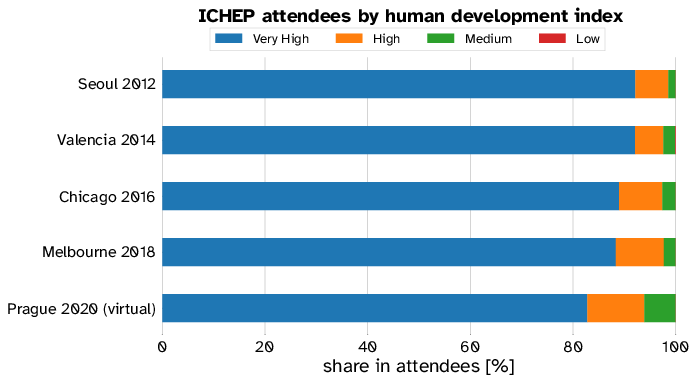
\includegraphics[width=1.\textwidth]{Sections/Figs/Travel/ICHEP_attendees.png}
    \caption[ICHEP participants by development index]%
        {The fraction of participants, categorised by human development index, HDI~\cite{hdiref} attending the last 5 instances of ICHEP.\label{fig:DevelopmentIndex}}
\end{figure}

%%%%%

\end{casestudy}

%%%%%

\begin{bestpractice}[Green travel top-ups on Erasmus+\label{bp:Erasmus}]{Green travel top-ups on Erasmus+}%
The EU mobility and training programme Erasmus+ has implemented funding top-ups for environmentally sustainable travel, which is more costly than point-to-point air travel in many instances, in particular between hubs for low-cost airline.  See \tref{tab:ErasmusGreenSupplement} for exact supplements for participants who receive travel funding, as excerpted from the 2022 programme guide~\cite{Erasmus+}). Moreover green travel over large distances can be more time-consuming. The programme allows for this by providing travel support for an additional 4 days of travel.

\ra{1.05}
\centering
\captionsetup{type=table}
\caption[Green travel supplements for Erasmus+ participants]{Green travel supplements for Erasmus+ participants receiving travel support.~\cite{Erasmus+}}
\label{tab:ErasmusGreenSupplement}
\begin{tabular}{@{}>{\baselineskip=10pt\centering\arraybackslash}p{3cm}>{\baselineskip=10pt\centering\arraybackslash}p{3cm}>{\baselineskip=10pt\centering\arraybackslash}p{3cm}@{}}
\toprule
    Travel distance\newline (km) & Standard travel \newline (EUR/participant) & Green travel \newline (EUR/participant)\\
    \midrule
    10 - 99 & 23  & \\
    100 - 499  & 180  & 210 \\
    500 - 1999  & 275  & 320 \\
    2000 - 2999  & 360  & 410 \\
    3000 - 3999  & 530  & 610 \\
    4000 - 7999  & 820  &  \\
    >8000  & 1500  &  \\
\bottomrule
\end{tabular}
\end{bestpractice}

%%%%%

\begin{bestpractice}[Internal regulations to reduce the impact of business travel at DESY\label{bp:DESY_travel}]{DESY sustainable travel regulations}%
    The regulations at DESY have been based on the goal of preserving the excellence of science and career opportunities while reacting to the necessity to save \CdO\ and other emissions. With its directive for business trips adopted in 2021, DESY relies on the climate policy principle Avoid - Reduce - Compensate.

    \textbf{Avoid:} The number of business trips will be reduced by 30\,\% compared to the situation before the start of the COVID-19 pandemic. This means that all travel planning is reviewed to identify whether the trip is needed to achieve the intended purpose, whether a virtual meeting could be just as beneficial, whether rotational changes between presence and digital are possible, and whether and how appointments can be bundled. In addition to \CdO\ savings and travel time, it should also be considered how much of the time spent traveling and for travel planning can actually be used as working time, and what costs are incurred or saved. Ultimately, digital meetings also contribute to a better flexibility of family and work life. They also reduce travel-related risks.

    \textbf{Reduce:} For some time now, it has already been possible to use the train instead of the plane, even if the costs were higher.  With the new directive, the use of the train is now mandatory if the destination can be reached within six hours total travel time. It should also be noted that the usable working time during the trip for rail travel is given as at least 50\;\% of the travel time (depending on the transfer frequency) and for flying it is assumed to be about 25\;\% of the travel time.

    \textbf{Compensate:} Until recently, compensation was not possible under the Federal Travel Expenses Act. However, since September 2020, there is a new regulation on the reimbursement policy for carbon offsets from the German ministry of science, whereby also grant recipients like DESY are allowed to offset their \CdO\ emissions for business trips. Starting in 2021, DESY will compensate the consequences of unavoidable air travel. There are established systems through which the climate-damaging effects of travel can be offset. The money goes to climate protection projects, including energy efficiency, biogas or biomass, solar energy, and environmental education. The selection of the compensation projects can be steered by DESY. 
\end{bestpractice}

%%%%%%%%%%%%%%%%%%%%%%%%%%%%%%%%%%%%%%%%%%%%%%%%%%

\begin{casestudy}[Cosmology from Home\footnote{This case study is, in part, adapted from the Cosmology from Home website~\cite{CfHwebsite}.}\label{cs:CfH}]{Cosmology from Home}%
Cosmology from Home (CfH)~\cite{CfHwebsite} is an "online by design" conference series that has been run on a yearly basis since 2020. It exploits the advantages of digital communication to accomplish things that have no analogue in traditional conference formats, while staying true to the dynamic and social nature of traditional conferences.

CfH is spread over two weeks, with two days per week dedicated to plenary and parallel talks. Talks are pre-recorded and shared with the conference participants ahead of the start of the conference. Other than a strict time limit, CfH places few constraints on the format of the talks. Participants are expected to watch the talks before the scheduled online discussion events. The discussions last a maximum of three hours per day to mitigate online fatigue, but multiple sessions can be scheduled to accommodate different time zones.

Other days are reserved for themed discussions, which are proposed by the participants.  Topics have included content related directly to cosmology, to scientific research more generally (i.e., technical or computational aspects), and social aspects, such as inclusivity and outreach in science.

The live discussions are hosted in virtual conference venue spaces to create a social atmosphere in which participants can wander around and join conversations. Suitable conference spaces are, \eg Sococo~\cite{Sococo}, Welo~\cite{Welo} and Gather~\cite{Gather}. In case the number of participants is such that the conference spaces are too small to host everyone at once, break-out rooms of a suitable video-conferencing platform can be used. In the specific case of CfH so far this has been Zoom~\cite{Zoom}.

CfH is coordinated asynchronously through an online message board, and a large part of the conference is dedicated to asynchronous text-based discussions. These discussions can start before the official opening of the conference and continue long after the conference has finished. In previous years, CfH used Slack~\cite{Slack}. (Alternatives include MatterMost~\cite{MatterMost}, Zulip~\cite{Zulip}, Microsoft Teams~\cite{Teams} or Discord~\cite{Discord}.) Discussion channels are grouped according to the scheduled live-talk discussion sessions (see below). Participants can discuss points in dedicated threads in these channels. Once a given discussion has grown sufficiently and has branched out into different sub-discussions, it can be given its own dedicated channel.

In addition to scheduled talk discussions, CfH implements scheduled themed discussions. These are moderated, workshop-style discussions on cosmological themes that are of interest to the conference participants. The topics are suggested, voted on and chosen via the Slack workspace. People can connect to the session via the conference space, but the main session is hosted in Zoom break-out rooms.

The final live discussion format featured by CfH is composed of spontaneous and unscheduled\footnote{“Unscheduled” means that the discussions are not part of the conference program. The participants can and do schedule these discussions on the asynchronous platform.} “informal” live discussions. The time allocated to the scheduled live discussions is limited, and the informal, breakaway sessions allow the participants to engage in more detailed explorations of topics.

The final live component of CfH consists of social events and interaction formats, such as social games and casual get-togethers, which complement the scientific discussion sessions on all days of the conference. These activities aim to reproduce (at least partially) the evening interactions of in-person conference social events.

One of the main advantages of the CfH format is the possibility for researchers to present and debate their work, and that of others, without the need for travel. This keeps the participation costs low and offers the potential for the conference to be carbon neutral or carbon negative (achieved, at present, through carbon offsetting of residual emissions).  The online format also makes the conference accessible to researchers from all over the world, subject to the availability of a suitable device and a stable internet connection by which to connect. The geographical distribution of participants in the previous three CfH conferences are shown in \fref{fig:CfH1}.

%%%%%

\begin{figure}
    \centering
    \captionsetup{type=figure}
    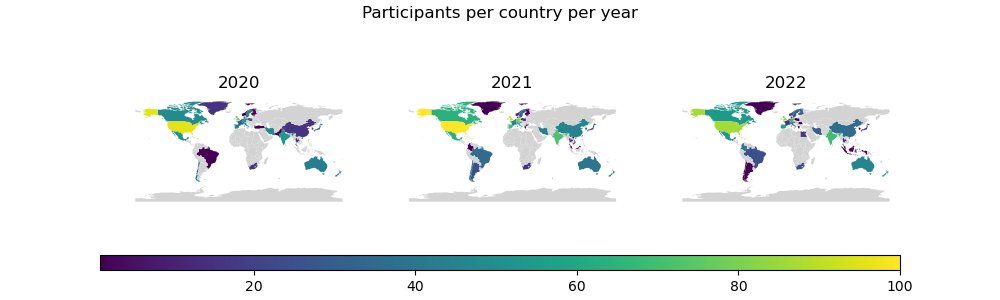
\includegraphics[width=1.\textwidth]{Sections/Figs/Travel/map.png}
    \caption[Geographical distribution of CfH participants for each of the installments by year.]%
        {Geographical distribution of Cosmology from Home participants for each of the installments by year.\label{fig:CfH1}}
\end{figure}

Additionally, participants can watch the talks according to their own schedules and personal obligations. Participants are able to pause and restart the talks, take time to digest them and to look up background material. They are also able to prepare and raise points for discussion in any of the conference environments. The asynchronous discussions can be tailored exactly to the schedule of the conference participants.

In the first CfH (2020), participants needed time to adjust to the format. This was to be expected, and the organisers actively encouraged participants to partake of the various aspects of the conference and actively modelled the expected social norms. The activity and enthusiasm of participation increased year on year. Speakers created innovative and accessible talk records, and participants regularly referred to these in the live and text-based discussions. Participants organised watch parties and impromptu discussions, made use of the various breakout rooms, and gathered in the virtual environments. The themed discussions proved to be particularly popular, and parallel sessions were often necessary to accommodate the high number of topic suggestions.

All participant feedback has been constructive and positive, and CfH has been well attended. The number of CfH participants were 255, 427 and 275 in 2020, 2021 and 2022, respectively~\cite{CfHwebsite}.  The format is easily tailored to various topics: a conference featuring this format in HEP is expected to be run late 2023.

\end{casestudy}


\end{document}
